\subsection{Dysgraphia}
Dysgraphia is a learning disability that primarily impacts a child's ability to write coherently and express their thoughts through written language. Individuals with dysgraphia may struggle with handwriting, spelling, grammar, and organizing their ideas on paper. In order to develop effective interventions for children with dysgraphia, it is important to understand their unique user profile. This includes identifying their specific goals, psychographics, problems, characteristics, and needs related to written expression and communication. Figure \ref{fig:disgrafiaUserProfile} displays the Dysgraphia user profile.

\begin{figure}[H]
    \centering
    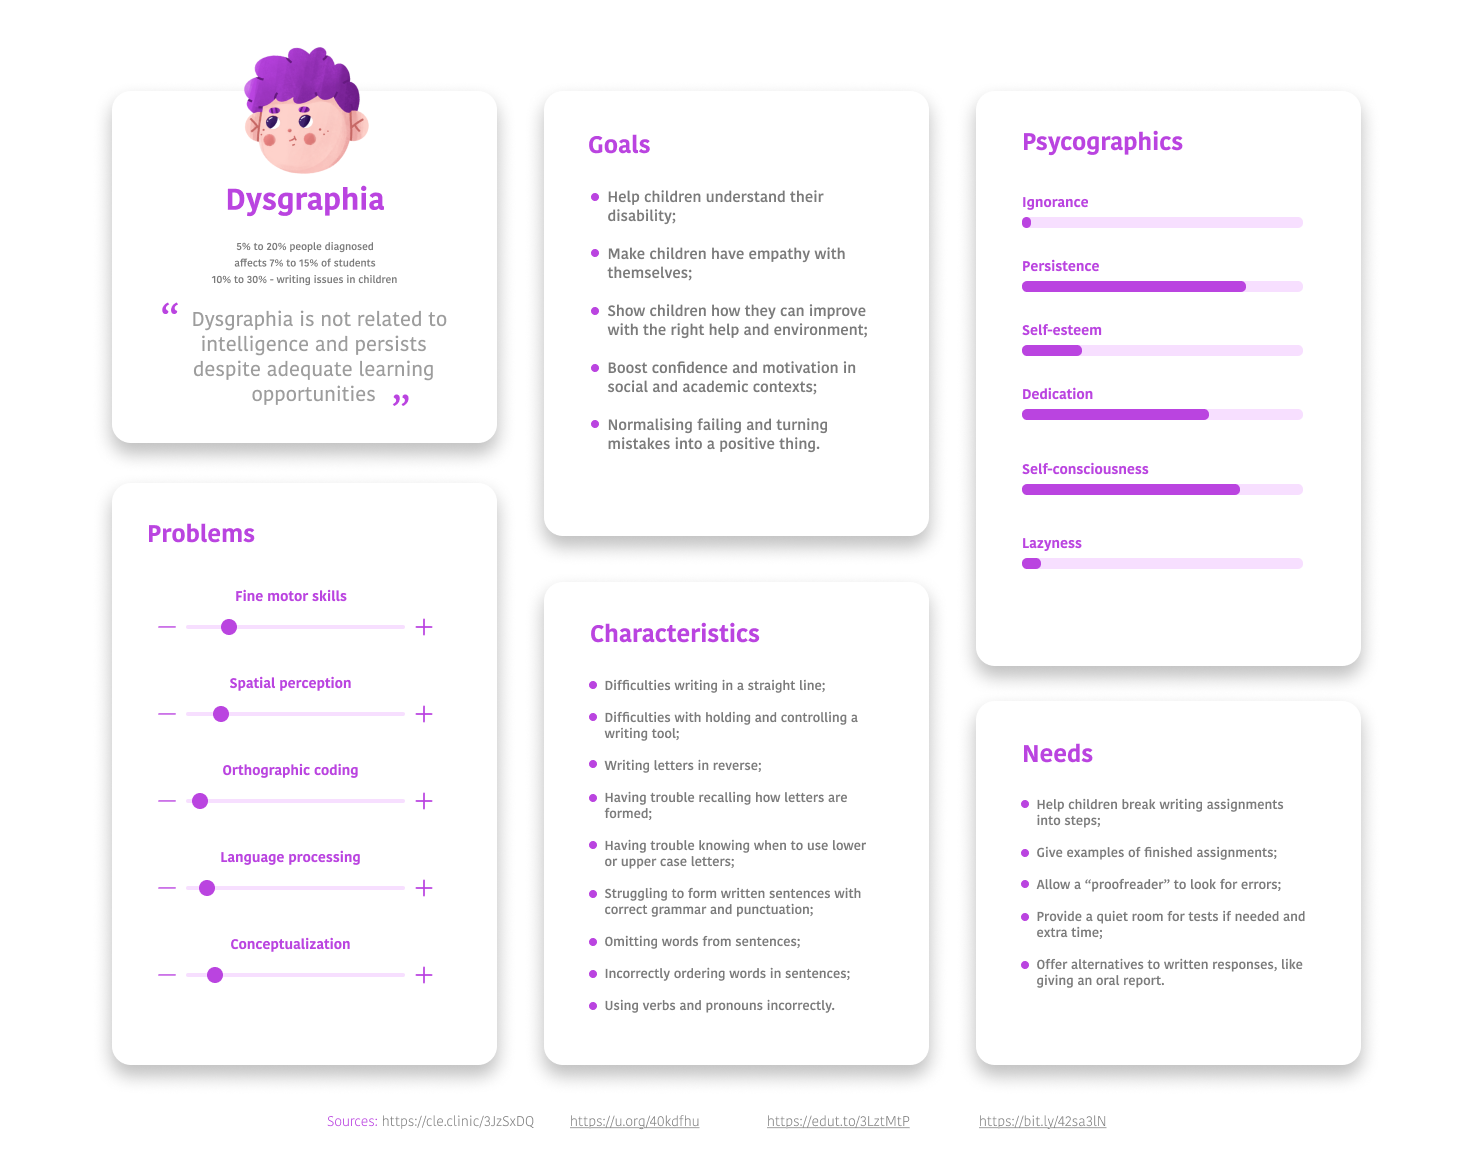
\includegraphics[width=1\linewidth]{Chapters/figma/Disgrafia.png}
    \caption{Dysgraphia User Profile}
    \label{fig:disgrafiaUserProfile}
\end{figure}

\paragraph{Goals}
\begin{itemize}
    \item \textbf{Help children understand their disability}: The mini-games aim to provide children with a comprehensive understanding of Dysgraphia, its impact on their writing skills, and the specific challenges they may face.
    \item \textbf{Foster empathy and self-acceptance}: By creating an environment of empathy and self-acceptance, the mini-games aim to help children develop a positive self-image, embrace their unique writing style, and build resilience in the face of writing difficulties.
    \item \textbf{Show children how they can improve}: The mini-games should demonstrate to children that with the right help, strategies, and supportive environment, they can improve their writing skills and overcome specific challenges related to Dysgraphia.
    \item \textbf{Boost confidence and motivation}: The mini-games aim to boost children's confidence in their writing abilities, celebrate their progress and achievements, and enhance their motivation to engage in writing tasks both in social and academic contexts.
    \item \textbf{Normalize failing and turning mistakes into a positive thing}: Creating a positive learning environment within the mini-games that encourages children to view mistakes as opportunities for growth and learning, fostering a growth mindset and resilience.
\end{itemize}

\paragraph{Psychographics}
\begin{itemize}
    \item \textbf{Low laziness}: Exhibiting a proactive and engaged attitude towards writing tasks.
    \item \textbf{Low ignorance}: Children with Dysgraphia generally have awareness of their writing difficulties and the challenges they face \cite{cleveland_dysgraphia}.
    \item \textbf{Low self-esteem}: Struggling with writing can negatively impact self-esteem and self-worth \cite{cleveland_dysgraphia}.
    \item \textbf{High persistence}: Demonstrating persistence and determination in overcoming writing challenges despite all the setbacks.
    \item \textbf{High dedication}: Displaying a strong commitment and effort in improving writing skills.
    \item \textbf{High self-consciousness}: Being self-conscious about their writing abilities in comparison to their peers.
\end{itemize}

\paragraph{Problems}
\begin{itemize}
    \item \textbf{Fine motor skills}: Difficulties in controlling and coordinating fine motor movements required for writing \cite{cleveland_dysgraphia}.
    \item \textbf{Spatial perception}: Challenges in perceiving and reproducing correct spacing, alignment, and proportions of letters and words on a page \cite{cleveland_dysgraphia}.
    \item \textbf{Orthographic coding}: Struggles in remembering and accurately reproducing the correct formation and shape of letters and words \cite{cleveland_dysgraphia}.
    \item \textbf{Language processing}: Difficulties in organizing and expressing thoughts in written form, including grammar, sentence structure, and punctuation \cite{cleveland_dysgraphia}.
    \item \textbf{Conceptualization}: Challenges in generating and organizing ideas coherently and effectively \cite{cleveland_dysgraphia}.
\end{itemize}

\paragraph{Characteristics}
\begin{itemize}
    \item \textbf{Difficulties writing on a straight line}: Struggling to maintain a consistent baseline or alignment while writing \cite{cleveland_dysgraphia}.
    \item \textbf{Difficulties with holding and controlling a writing tool}: Challenges in gripping and controlling the pen or pencil while writing \cite{understood_accommodations}.
    \item \textbf{Writing letters in reverse}: Frequently reversing or inverting letters or numbers \cite{pmc_dysgraphia}.
    \item \textbf{Trouble recalling letter formation}: Difficulty on remembering and reproducing the proper formation of letters \cite{edutopia_dysgraphia}.
    \item \textbf{Difficulty with capitalization}: Confusion regarding when to use uppercase or lowercase letters \cite{cleveland_dysgraphia}.
    \item \textbf{Struggling with grammar and punctuation}: Difficulties in using correct grammar, punctuation, and sentence structure \cite{cleveland_dysgraphia}.
    \item \textbf{Omitting or misordering words}: Frequently leaving out words or rearranging them incorrectly within sentences \cite{cleveland_dysgraphia}.
    \item \textbf{Incorrect verb and pronoun usage}: Using verbs and pronouns incorrectly, leading to grammatical errors \cite{cleveland_dysgraphia}.
\end{itemize}

\paragraph{Needs}
\begin{itemize}
    \item \textbf{Breaking writing assignments into steps}: Providing clear and structured instructions, breaking down writing tasks into manageable steps to enhance organization and reduce overwhelm \cite{understood_accommodations}.
    \item \textbf{Providing examples of finished assignments}: Offering visual models and examples of well-organized and properly completed assignments helps to understand expectations \cite{understood_accommodations}.
    \item \textbf{Allowing a ''proofreader'' to look for errors}: Incorporating a feature within the mini-games that allows children to have their written work reviewed by a virtual or real person to identify and correct errors, providing feedback and guidance \cite{understood_accommodations}.
    \item \textbf{Providing a quiet room for tests if needed and extra time}: Recognizing the potential impact of environmental distractions on writing performance and offering a quiet and focused space for assessments, along with appropriate time extensions to accommodate the specific needs of children with Dysgraphia \cite{understood_accommodations}.
    \item \textbf{Offering alternatives to written responses}: Recognizing that writing may pose significant challenges for children with Dysgraphia, the mini-games should provide opportunities for alternative modes of expression, such as giving oral reports or utilizing multimedia formats \cite{understood_accommodations}.
\end{itemize}